\documentclass[mstat,12pt]{unswthesis}

\usepackage{color}
\usepackage{fancyvrb}
\newcommand{\VerbBar}{|}
\newcommand{\VERB}{\Verb[commandchars=\\\{\}]}
\DefineVerbatimEnvironment{Highlighting}{Verbatim}{commandchars=\\\{\}}
% Add ',fontsize=\small' for more characters per line
\usepackage{framed}
\definecolor{shadecolor}{RGB}{248,248,248}
\newenvironment{Shaded}{\begin{snugshade}}{\end{snugshade}}
\newcommand{\AlertTok}[1]{\textcolor[rgb]{0.94,0.16,0.16}{#1}}
\newcommand{\AnnotationTok}[1]{\textcolor[rgb]{0.56,0.35,0.01}{\textbf{\textit{#1}}}}
\newcommand{\AttributeTok}[1]{\textcolor[rgb]{0.77,0.63,0.00}{#1}}
\newcommand{\BaseNTok}[1]{\textcolor[rgb]{0.00,0.00,0.81}{#1}}
\newcommand{\BuiltInTok}[1]{#1}
\newcommand{\CharTok}[1]{\textcolor[rgb]{0.31,0.60,0.02}{#1}}
\newcommand{\CommentTok}[1]{\textcolor[rgb]{0.56,0.35,0.01}{\textit{#1}}}
\newcommand{\CommentVarTok}[1]{\textcolor[rgb]{0.56,0.35,0.01}{\textbf{\textit{#1}}}}
\newcommand{\ConstantTok}[1]{\textcolor[rgb]{0.00,0.00,0.00}{#1}}
\newcommand{\ControlFlowTok}[1]{\textcolor[rgb]{0.13,0.29,0.53}{\textbf{#1}}}
\newcommand{\DataTypeTok}[1]{\textcolor[rgb]{0.13,0.29,0.53}{#1}}
\newcommand{\DecValTok}[1]{\textcolor[rgb]{0.00,0.00,0.81}{#1}}
\newcommand{\DocumentationTok}[1]{\textcolor[rgb]{0.56,0.35,0.01}{\textbf{\textit{#1}}}}
\newcommand{\ErrorTok}[1]{\textcolor[rgb]{0.64,0.00,0.00}{\textbf{#1}}}
\newcommand{\ExtensionTok}[1]{#1}
\newcommand{\FloatTok}[1]{\textcolor[rgb]{0.00,0.00,0.81}{#1}}
\newcommand{\FunctionTok}[1]{\textcolor[rgb]{0.00,0.00,0.00}{#1}}
\newcommand{\ImportTok}[1]{#1}
\newcommand{\InformationTok}[1]{\textcolor[rgb]{0.56,0.35,0.01}{\textbf{\textit{#1}}}}
\newcommand{\KeywordTok}[1]{\textcolor[rgb]{0.13,0.29,0.53}{\textbf{#1}}}
\newcommand{\NormalTok}[1]{#1}
\newcommand{\OperatorTok}[1]{\textcolor[rgb]{0.81,0.36,0.00}{\textbf{#1}}}
\newcommand{\OtherTok}[1]{\textcolor[rgb]{0.56,0.35,0.01}{#1}}
\newcommand{\PreprocessorTok}[1]{\textcolor[rgb]{0.56,0.35,0.01}{\textit{#1}}}
\newcommand{\RegionMarkerTok}[1]{#1}
\newcommand{\SpecialCharTok}[1]{\textcolor[rgb]{0.00,0.00,0.00}{#1}}
\newcommand{\SpecialStringTok}[1]{\textcolor[rgb]{0.31,0.60,0.02}{#1}}
\newcommand{\StringTok}[1]{\textcolor[rgb]{0.31,0.60,0.02}{#1}}
\newcommand{\VariableTok}[1]{\textcolor[rgb]{0.00,0.00,0.00}{#1}}
\newcommand{\VerbatimStringTok}[1]{\textcolor[rgb]{0.31,0.60,0.02}{#1}}
\newcommand{\WarningTok}[1]{\textcolor[rgb]{0.56,0.35,0.01}{\textbf{\textit{#1}}}}


%%%%%%%%%%%%%%%%%%%%%%%%%%%%%%%%%%%%%%%%%%%%%%%%%%%%%%%%%%%%%%%%%%
% 
% OK...Now we get to some actual input.  The first part sets up
% the title etc that will appear on the front page
%
%%%%%%%%%%%%%%%%%%%%%%%%%%%%%%%%%%%%%%%%%%%%%%%%%%%%%%%%%%%%%%%%%

\title{Capstone Project by Team D\\[0.5cm]A Data Science Approach to Forecasting Electricity Demand in NSW,
Australia}

\authornameonly{Baheerathan Gnanasundram, Matthew Seery, Mohammad Ahsan Ullah, Rahul Lobo. }

\author{\Authornameonly}

\copyrightfalse
\figurespagefalse
\tablespagefalse

%%%%%%%%%%%%%%%%%%%%%%%%%%%%%%%%%%%%%%%%%%%%%%%%%%%%%%%%%%%%%%%%%
%
%  And now the document begins
%  The \beforepreface and \afterpreface commands puts the
%  contents page etc in
%
%%%%%%%%%%%%%%%%%%%%%%%%%%%%%%%%%%%%%%%%%%%%%%%%%%%%%%%%%%%%%%%%%%


%%%%%%%%%%%%%%%%%%%%%%%%%%%%%%%%%%%%%%%%%%%%%%%%%%%%%%%%%%%%%%%%%%%%%%%
%
%  A small sample UNSW Coursework Masters thesis file.
%  Any questions to Ian Doust i.doust@unsw.edu.au and/or Gery Geenens ggeenens@unsw.edu.au
%
%%%%%%%%%%%%%%%%%%%%%%%%%%%%%%%%%%%%%%%%%%%%%%%%%%%%%%%%%%%%%%%%%%%%%%%
%
%  The first part pulls in a UNSW Thesis class file.  This one is
%  slightly nonstandard and has been set up to do a couple of
%  things automatically
%
 
%%%%%%%%%%%%%%%%%
%% Precisely one of the next four lines should be uncommented.
%% Choose the one which matches your degree, uncomment it, and comment out the other two!
%\documentclass[mfin,12pt]{unswthesis}    %%  For Master of Financial Mathematics 
%\documentclass[mmath,12pt]{unswthesis}   %%  For Master of Mathematics
%\documentclass[mstat,12pt]{unswthesis}  %%  For Master of Statistics
%%%%%%%%%%%%%%%%%



\linespread{1}
\usepackage{amsfonts}
\usepackage{amssymb}
\usepackage{amsthm}
\usepackage{latexsym,amsmath}
\usepackage{graphicx}
\usepackage{afterpage}
\usepackage[colorlinks]{hyperref}
 \hypersetup{
     colorlinks=true,
     linkcolor=blue,
     filecolor=blue,
     citecolor= black,      
     urlcolor=cyan,
     }
\usepackage{textcomp}
\usepackage{longtable}
\usepackage{booktabs}
\usepackage{float}

%%%%%%%%%%%%%%%%%%%%%%%%%%%%%%%%%%%%%%%%%%%%%%%%%%%%%%%%%%%%%%%%%
%
%  The following are some simple LaTeX macros to give some
%  commonly used letters in funny fonts. You may need more or less of
%  these
%
\newcommand{\R}{\mathbb{R}}
\newcommand{\Q}{\mathbb{Q}}
\newcommand{\C}{\mathbb{C}}
\newcommand{\N}{\mathbb{N}}
\newcommand{\F}{\mathbb{F}}
\newcommand{\PP}{\mathbb{P}}
\newcommand{\T}{\mathbb{T}}
\newcommand{\Z}{\mathbb{Z}}
\newcommand{\B}{\mathfrak{B}}
\newcommand{\BB}{\mathcal{B}}
\newcommand{\M}{\mathfrak{M}}
\newcommand{\X}{\mathfrak{X}}
\newcommand{\Y}{\mathfrak{Y}}
\newcommand{\CC}{\mathcal{C}}
\newcommand{\E}{\mathbb{E}}
\newcommand{\cP}{\mathcal{P}}
\newcommand{\cS}{\mathcal{S}}
\newcommand{\A}{\mathcal{A}}
\newcommand{\ZZ}{\mathcal{Z}}
%%%%%%%%%%%%%%%%%%%%%%%%%%%%%%%%%%%%%%%%%%%%%%%%%%%%%%%%%%%%%%%%%%%%%
%
% The following are much more esoteric commands that I have left in
% so that this file still processes. Use or delete as you see fit
%
\newcommand{\bv}[1]{\mbox{BV($#1$)}}
\newcommand{\comb}[2]{\left(\!\!\!\begin{array}{c}#1\\#2\end{array}\!\!\!\right)
}
\newcommand{\Lat}{{\rm Lat}}
\newcommand{\var}{\mathop{\rm var}}
\newcommand{\Pt}{{\mathcal P}}
\def\tr(#1){{\rm trace}(#1)}
\def\Exp(#1){{\mathbb E}(#1)}
\def\Exps(#1){{\mathbb E}\sparen(#1)}
\newcommand{\floor}[1]{\left\lfloor #1 \right\rfloor}
\newcommand{\ceil}[1]{\left\lceil #1 \right\rceil}
\newcommand{\hatt}[1]{\widehat #1}
\newcommand{\modeq}[3]{#1 \equiv #2 \,(\text{mod}\, #3)}
\newcommand{\rmod}{\,\mathrm{mod}\,}
\newcommand{\p}{\hphantom{+}}
\newcommand{\vect}[1]{\mbox{\boldmath $ #1 $}}
\newcommand{\reff}[2]{\ref{#1}.\ref{#2}}
\newcommand{\psum}[2]{\sum_{#1}^{#2}\!\!\!'\,\,}
\newcommand{\bin}[2]{\left( \begin{array}{@{}c@{}}
				#1 \\ #2
			\end{array}\right)	}
%
%  Macros - some of these are in plain TeX (gasp!)
%
\newcommand{\be}{($\beta$)}
\newcommand{\eqp}{\mathrel{{=}_p}}
\newcommand{\ltp}{\mathrel{{\prec}_p}}
\newcommand{\lep}{\mathrel{{\preceq}_p}}
\def\brack#1{\left \{ #1 \right \}}
\def\bul{$\bullet$\ }
\def\cl{{\rm cl}}
\let\del=\partial
\def\enditem{\par\smallskip\noindent}
\def\implies{\Rightarrow}
\def\inpr#1,#2{\t \hbox{\langle #1 , #2 \rangle} \t}
\def\ip<#1,#2>{\langle #1,#2 \rangle}
\def\lp{\ell^p}
\def\maxb#1{\max \brack{#1}}
\def\minb#1{\min \brack{#1}}
\def\mod#1{\left \vert #1 \right \vert}
\def\norm#1{\left \Vert #1 \right \Vert}
\def\paren(#1){\left( #1 \right)}
\def\qed{\hfill \hbox{$\Box$} \smallskip}
\def\sbrack#1{\Bigl \{ #1 \Bigr \} }
\def\ssbrack#1{ \{ #1 \} }
\def\smod#1{\Bigl \vert #1 \Bigr \vert}
\def\smmod#1{\bigl \vert #1 \bigr \vert}
\def\ssmod#1{\vert #1 \vert}
\def\sspmod#1{\vert\, #1 \, \vert}
\def\snorm#1{\Bigl \Vert #1 \Bigr \Vert}
\def\ssnorm#1{\Vert #1 \Vert}
\def\sparen(#1){\Bigl ( #1 \Bigr )}

\newcommand\blankpage{%
    \null
    \thispagestyle{empty}%
    \addtocounter{page}{-1}%
    \newpage}

%%%%%%%%%%%%%%%%%%%%%%%%%%%%%%%
%
% These environments allow you to get nice numbered headings
%  for your Theorems, Definitions etc.  
%
%  Environments
%
%%%%%%%%%%%%%%%%%%%%%%%%%%%%%%%

\newtheorem{theorem}{Theorem}[section]
\newtheorem{lemma}[theorem]{Lemma}
\newtheorem{proposition}[theorem]{Proposition}
\newtheorem{corollary}[theorem]{Corollary}
\newtheorem{conjecture}[theorem]{Conjecture}
\newtheorem{definition}[theorem]{Definition}
\newtheorem{example}[theorem]{Example}
\newtheorem{remark}[theorem]{Remark}
\newtheorem{question}[theorem]{Question}
\newtheorem{notation}[theorem]{Notation}
\numberwithin{equation}{section}

%%%%%%%%%%%%%%%%%%%%%%%%%%%%%%%%%%%%%%%%%%%%%%%%%%%%%%%%%%%%%%%%%%
%
%  If you've got some funny special words that LaTeX might not
% hyphenate properly, you can give it a helping hand:
%

\hyphenation{Mar-cin-kie-wicz Rade-macher}






\begin{document}

\beforepreface

%\afterpage{\blankpage}

% plagiarism

\prefacesection{Plagiarism statement}

\vskip 2pc \noindent I declare that this thesis is my
own work, except where acknowledged, and has not been submitted for
academic credit elsewhere. 

\vskip 2pc  \noindent I acknowledge that the assessor of this
thesis may, for the purpose of assessing it:
\begin{itemize}
\item Reproduce it and provide a copy to another member of the University; and/or,
\item Communicate a copy of it to a plagiarism checking service (which may then retain a copy of it on its database for the purpose of future plagiarism checking).
\end{itemize}

\vskip 2pc \noindent I certify that I have read and understood the University Rules in
respect of Student Academic Misconduct, and am aware of any potential plagiarism penalties which may 
apply.\vspace{24pt}

\vskip 2pc \noindent By signing 
this declaration I am
agreeing to the statements and conditions above.
\vskip 2pc \noindent
Signed: \rule{7cm}{0.25pt} \hfill Date: \rule{4cm}{0.25pt} \\[1cm]
Signed: \rule{7cm}{0.25pt} \hfill Date: \rule{4cm}{0.25pt} \\[1cm]
Signed: \rule{7cm}{0.25pt} \hfill Date: \rule{4cm}{0.25pt} \\[1cm]
Signed: \rule{7cm}{0.25pt} \hfill Date: \rule{4cm}{0.25pt} \\[1cm]
\vskip 1pc

%\afterpage{\blankpage}

% Acknowledgements are optional


\prefacesection{Acknowledgements}

{\bigskip}All thanks must go to our families and university professors who have
guided us through this Capstone Project. Without them this would not be
possible.\\[1cm] 

{\bigskip\bigskip\bigskip\noindent} 15/06/2021.

%\afterpage{\blankpage}

% Abstract

\prefacesection{Abstract}

Forecasting electricity demand is an important requirement as there are
now more interested stakeholders associated with the generation and
distribution of this service. Traditionally electricity demand was just
the concern of governments. However, this has now been extended to
market bodies and owners and operators of the underlying infrastructure
required for this service. Forecasting accurate energy demand not only
supports network infrastructure, but also aides investment decisions
about power generation. It is of thus of interest to a variety of
stakeholders including power utilities, energy policymakers, and private
investors just to name a few. This study aims to demonstrate how neural
network (specifically LSTM neural networks) can be used to accurately
forecast short-term energy demand. The focus will be on attributes such
as temperature, month of the year, day of the week and time of the day
as well as how past time lags can be used to predict future demand
values. It is envisaged that the results of this study will provide
useful insights for governments and market bodies to assist in the
rules, policies and pricing that are invoked on the energy sector.
Additionally, the businesses operating in this sector can use this
information to guide their decision-making regarding electricity
generation and distribution, as well as for the purpose of price
benchmarking.

%\afterpage{\blankpage}


\afterpreface





%%%%%%%%%%%%%%%%%%%%%%%%%%%%%%%%%%%%%%%%%%%%%%%%%%%%%%%%%%%%%%%%%%
%
% Now we can start on the first chapter
% Within chapters we have sections, subsections and so forth
%
%%%%%%%%%%%%%%%%%%%%%%%%%%%%%%%%%%%%%%%%%%%%%%%%%%%%%%%%%%%%%%%%%%



%%%%%%%%%%%%%%%%%%%%%%%%%%%%%%%%%%%%%

%\afterpage{\blankpage}


\hypertarget{introduction}{%
\chapter{Introduction}\label{introduction}}

Towards the end of the 20th century, countries throughout the world
began moving away from regulated government-controlled energy supply to
a deregulated sector influenced by market forces \cite{Catalao2007}.
This means that forecasting for electricity demands is essential
information required beyond previously regulated governmental
structures. It is now required by the market bodies working in the
sector and private industries who invest in the generation and
distribution of electricity. In turn, this aids in better rules,
policies, and pricing in the energy sector. However, for this study, the
focus will primarily be on short-term forecasting as this can greatly
aid vested parties concerned in maximising profits and cutting costs.

\bigskip

Temperature plays a significant role in electricity demand. This is
because heating is utilised more by customers in the cooler months while
cooling is required for the hottest months of the year. For that reason,
temperature is an essential attribute that will be investigated in this
study. However, temperature does not account for other factors such as
humidity or varying electricity usage patterns associated with specific
days of the weeks. For example, a temperature of 25 degrees in Spring
may not lead to as much usage of air conditioning as a humid day in
Summer with the same temperature. Additionally, the rate of usage of
electricity will inevitably vary between weekdays, weekends, and public
holidays due to the varying ratios of usage between business and
residential customers. Therefore, the month of the year, day of the week
and time of day will also be examined in this study.

\hypertarget{literature-review}{%
\chapter{Literature Review}\label{literature-review}}

There have been various studies undertaken where more traditional
statistical methods such as multiple linear regression (MLR) have been
utilised to predict demand \cite{Mohamed2005}. However, in more recent
times there has been greater focus on the use of neural networks to help
solve the problem of forecasting demand \cite{Gonzalez2008}. The
advantage of neural networks is they are very suitable for determining
non-linear relationships \cite{Gonzalez2008} and have been widely used
for short-term demand forecasting \cite{Ciulla2019}. They are also very
flexible and easy to configure when dealing with time-series data
\cite{Carmona2002}. For neural networks, monthly values have been a
popular unit of measure and this is particularly true when short-term
forecasting of demand has been employed \cite{Carmona2002}. However,
this proposed solution differs because the focus will be on intervals
shorter than even a day as this is of greater interest to the client.
Nevertheless, the month of the year will still be considered as an input
factor for the model for its potential to distinguish factors such as
humidity that are not fully explained by temperature alone. Another
distinguishing factor for this study will be the emphasis on the day of
the week where each record will be categorised as either a weekday,
weekend, or public holiday.

\bigskip

Up until the time of writing, the majority of deep learning models being
appliied to energy forecasting fall under the subset of three major ways
\cite{Kumar2013}. These are: A feed forward neural network (FFNN)/Multi
Layer Perceptron (MLP) through the process of increasing the number of
hidden layers, some form of recurrence through a recurrent neural
network (RNN), long-short term memory (LSTM) or gated recurrent unit
(GRU), or through sequentially combining different types of algorithms
into an overall structure. In 2020, Xue et al.~contrasted these
different approaches in order to forecast the heating demand of a
district system \cite{Xue2020}. Their experiments showed that the LSTM
models were among the highest-performing models tested for.

\bigskip

When applied to natural gas forecasting, a close relative to electricity
demand, RNN models have proven to be useful in prediction. Wei et
al.~(2019) explored the application of LSTM for forecasting natural gas
consumption of four cities \cite{Xue2020}. In addition, LSTM models used
for forecasting were compared with other model techniques, including
multiple linear regression, feed-forward neural networks, and a support
vector regression in this study. The authors' rigorous testing
demonstrated that LSTM models achieved a greater accuracy than the other
data-driven models. It appears that RNN and LSTM models have formed the
majority of accurate forecasting implementations to date, with other
machine learning techniques such as SVMs performing as well as, but not
better than RNN and LSTM based models. An example of this is
demonstrated by Amarasignhe et al.~(2017), who contrasted the deep
learning techniques of a Convolutional Neural Network (CNN) and LSTM,
against a traditional machine learning technique (SVM) in order to
forecast the energy demand of a building. This forecast was for a time
period of sixty hours ahead and used 4 years of training data
\cite{Amarasinghe2016}. Their experiments proved that the deep learning
based forecasting models obtained less forecasting error when compared
with standard machine learning-based techniques; in particular, the LSTM
obtained the smallest error.

\bigskip

Due to the significance of the LSTM accuracy across a variety of these
studies, it will form the basis of this analysis.

\hypertarget{material-and-methods}{%
\chapter{Material and Methods}\label{material-and-methods}}

\hypertarget{software}{%
\section{Software}\label{software}}

R and Python of course are great software for Data Science. Sometimes,
you might want to use \texttt{bash} utilities such as \texttt{awk} or
\texttt{sed}.

Of course, to ensure reproducibility, you should use something like
\texttt{Git} and RMarkdown (or a Jupyter Notebook). Do \textbf{not} use
Word!

\hypertarget{description-of-the-data}{%
\section{Description of the Data}\label{description-of-the-data}}

How are the data stored? What are the sizes of the data files? How many
files? etc.

\hypertarget{pre-processing-steps}{%
\section{Pre-processing Steps}\label{pre-processing-steps}}

What did you have to do to transform the data so that they become
useable?

\hypertarget{data-cleaning}{%
\section{Data Cleaning}\label{data-cleaning}}

How did you deal with missing data? etc.

\hypertarget{assumptions}{%
\section{Assumptions}\label{assumptions}}

What assumptions are you making on the data?

\hypertarget{modelling-methods}{%
\section{Modelling Methods}\label{modelling-methods}}

\hypertarget{exploratory-data-analysis}{%
\chapter{Exploratory Data Analysis}\label{exploratory-data-analysis}}

This is where you explore your data using histograms, scatterplots,
boxplots, numerical summaries, etc.

\hypertarget{using-r}{%
\section{Using R}\label{using-r}}

\begin{Shaded}
\begin{Highlighting}[]
\KeywordTok{boxplot}\NormalTok{(cars, }\DataTypeTok{col =} \KeywordTok{c}\NormalTok{(}\StringTok{"#5975a4"}\NormalTok{, }\StringTok{"#cc8963"}\NormalTok{))}
\end{Highlighting}
\end{Shaded}

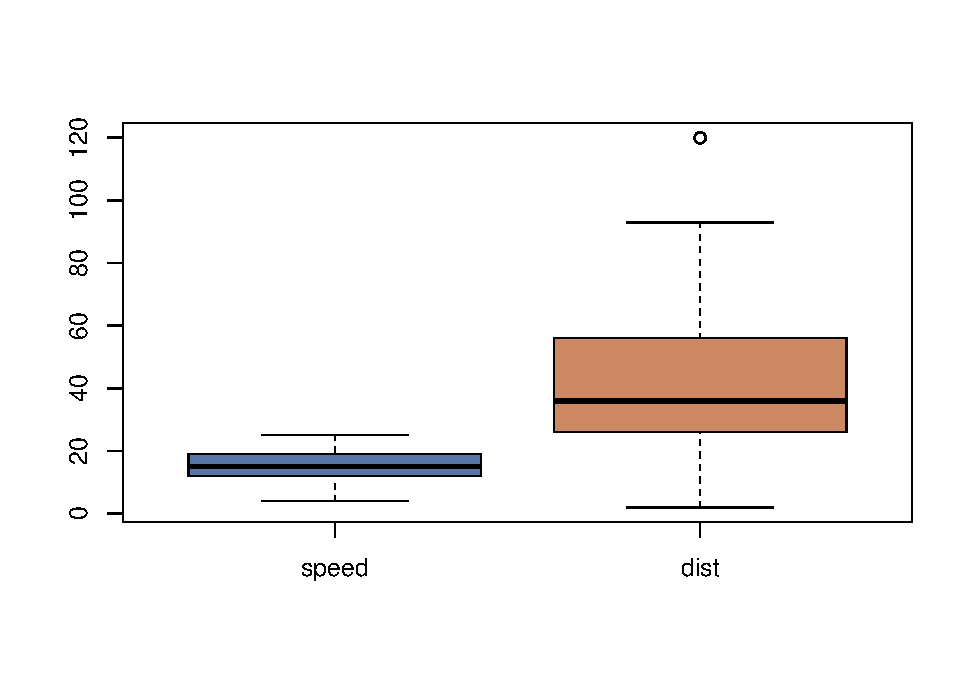
\includegraphics{unsw-ZZSC9020-report_files/figure-latex/unnamed-chunk-1-1.pdf}

\hypertarget{using-python}{%
\section{Using Python}\label{using-python}}

See
\url{https://cran.r-project.org/web/packages/reticulate/vignettes/r_markdown.html}
for more details.

\bigskip

You need to install the R package \texttt{reticulate}.

\begin{Shaded}
\begin{Highlighting}[]
\BuiltInTok{print}\NormalTok{(}\StringTok{"Python can be used with MATHxxxx!"}\NormalTok{)}
\end{Highlighting}
\end{Shaded}

\begin{verbatim}
## Python can be used with MATHxxxx!
\end{verbatim}

\begin{Shaded}
\begin{Highlighting}[]
\ImportTok{import}\NormalTok{ sys}
\BuiltInTok{print}\NormalTok{(sys.version)}
\end{Highlighting}
\end{Shaded}

\begin{verbatim}
## 3.6.12 |Anaconda, Inc.| (default, Sep  9 2020, 00:29:25) [MSC v.1916 64 bit (AMD64)]
\end{verbatim}

\begin{Shaded}
\begin{Highlighting}[]
\ImportTok{import}\NormalTok{ numpy }\ImportTok{as}\NormalTok{ np}
\NormalTok{np.random.seed(}\DecValTok{1}\NormalTok{)}
\NormalTok{np.random.normal(}\FloatTok{0.0}\NormalTok{, }\FloatTok{1.0}\NormalTok{, size}\OperatorTok{=}\DecValTok{10}\NormalTok{)}
\end{Highlighting}
\end{Shaded}

\begin{verbatim}
## array([ 1.62434536, -0.61175641, -0.52817175, -1.07296862,  0.86540763,
##        -2.3015387 ,  1.74481176, -0.7612069 ,  0.3190391 , -0.24937038])
\end{verbatim}

\begin{Shaded}
\begin{Highlighting}[]
\ImportTok{import}\NormalTok{ pandas }\ImportTok{as}\NormalTok{ pd}
\ImportTok{import}\NormalTok{ matplotlib.pyplot }\ImportTok{as}\NormalTok{ plt}
\NormalTok{df}\OperatorTok{=}\NormalTok{pd.DataFrame([[}\DecValTok{1}\NormalTok{, }\DecValTok{2}\NormalTok{], [}\DecValTok{3}\NormalTok{, }\DecValTok{4}\NormalTok{], [}\DecValTok{4}\NormalTok{, }\DecValTok{3}\NormalTok{], [}\DecValTok{2}\NormalTok{, }\DecValTok{3}\NormalTok{]])}
\NormalTok{fig }\OperatorTok{=}\NormalTok{ plt.figure(figsize}\OperatorTok{=}\NormalTok{(}\DecValTok{4}\NormalTok{, }\DecValTok{4}\NormalTok{))}
\ControlFlowTok{for}\NormalTok{ i }\KeywordTok{in}\NormalTok{ df.columns:}
\NormalTok{    ax}\OperatorTok{=}\NormalTok{plt.subplot(}\DecValTok{2}\NormalTok{,}\DecValTok{1}\NormalTok{,i}\OperatorTok{+}\DecValTok{1}\NormalTok{) }
\NormalTok{    df[[i]].plot(ax}\OperatorTok{=}\NormalTok{ax)}
    \BuiltInTok{print}\NormalTok{(i)}
\end{Highlighting}
\end{Shaded}

\begin{verbatim}
## <AxesSubplot:>
## 0
## <AxesSubplot:>
## 1
\end{verbatim}

\begin{Shaded}
\begin{Highlighting}[]
\NormalTok{plt.show()}
\end{Highlighting}
\end{Shaded}

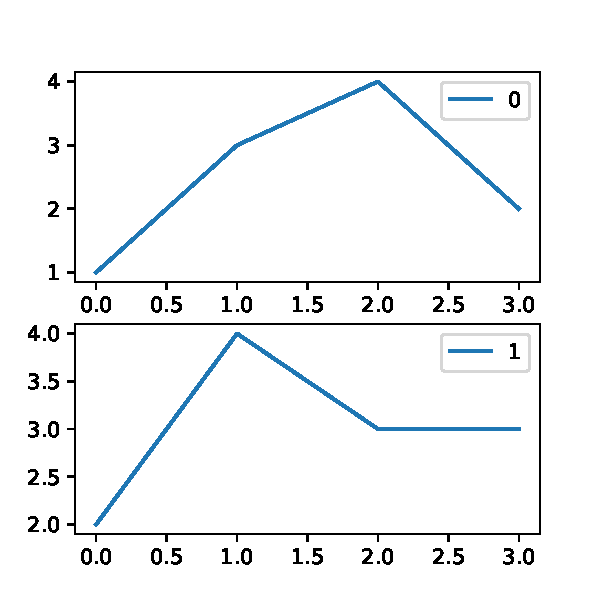
\includegraphics{unsw-ZZSC9020-report_files/figure-latex/unnamed-chunk-2-1.pdf}

\hypertarget{analysis-and-results}{%
\chapter{Analysis and Results}\label{analysis-and-results}}

\hypertarget{a-first-model}{%
\section{A First Model}\label{a-first-model}}

Having a very simple model is always good so that you can benchmark any
result you would obtain with a more elaborate model.

\bigskip

For example, one can use the linear regression model

\[
Y_i = \beta_0 + \beta_1 x_{1i} + \cdots \beta_p x_{pi} + \epsilon_i, \qquad i=1,\ldots,n.
\] where it is assumed that the \(\epsilon_i\)'s are i.i.d.~\(N(0,1)\).

\hypertarget{discussion}{%
\chapter{Discussion}\label{discussion}}

Put the results you got in the previous chapter in perspective with
respect to the problem studied.

\hypertarget{conclusion-and-further-issues}{%
\chapter{Conclusion and Further
Issues}\label{conclusion-and-further-issues}}

What are the main conclusions? What are your recommendations for the
``client''? What further analysis could be done in the future?

A figure:

\begin{figure}[H]

\includegraphics{unsw-logo.png}
\caption{A caption}\label{myfigure}
\end{figure}

In the text, see Figure \ref{myfigure}.

\bibliographystyle{elsarticle-num}
\bibliography{references}

\hypertarget{appendix}{%
\chapter*{Appendix}\label{appendix}}
\addcontentsline{toc}{chapter}{Appendix}

\hypertarget{codes}{%
\section*{\texorpdfstring{\textbf{Codes}}{Codes}}\label{codes}}
\addcontentsline{toc}{section}{\textbf{Codes}}

Add you codes here.

\hypertarget{tables}{%
\section*{\texorpdfstring{\textbf{Tables}}{Tables}}\label{tables}}
\addcontentsline{toc}{section}{\textbf{Tables}}

If you have tables, you can add them here.

Use \url{https://www.tablesgenerator.com/markdown_tables} to crete very
simple markdown tables, otherwise use \LaTeX.

\begin{longtable}[]{@{}lcr@{}}
\toprule
Tables & Are & Cool\tabularnewline
\midrule
\endhead
col 1 is & left-aligned & \$1600\tabularnewline
col 2 is & centered & \$12\tabularnewline
col 3 is & right-aligned & \$1\tabularnewline
\bottomrule
\end{longtable}







\end{document}


